%!TEX root = ../Main.tex

\section{Methodology and Data}
\subsection{Methodology: Linear Regression and HAR-RV model}
\begin{itemize}\itemsep0pt
\item Reg1: without VIX
\begin{itemize}\itemsep0pt
\item Reg1a: regress realized volatility on historic volatility using simple linear regression
\item Reg1b: regress realized volatility on historic volatility using HAR-RV model
\end{itemize}
\item Reg2: with VIX
\begin{itemize}
\item Reg2b: regress realized volatility on historic volatility using simple linear regression
\item Reg2b: regress realized volatility on historic volatility using HAR-RV model
\end{itemize}
\end{itemize}
%
\begin{flalign}
&\sigma_{t,x}^{RV} = \alpha_{x,t} + \beta_{x,t}^{HV} \sigma_{x,t}^{HV}\\
&\sigma_{x,t}^{RV} = \alpha_{x,t} + \beta_{x,t}^{HV,d} \sigma_{x,t}^{HV,d} + \beta_{x,t}^{HV,w} \sigma_{x,t}^{HV,w} + \beta_{x,t}^{HV,m} \sigma_{x,t}^{HV,m}\\
&\sigma_{x,t}^{RV} = \alpha_{x,t} + \beta_{x,t}^{HV} \sigma_{x,t}^{HV} + \beta_{x,t}^{VIX} + \sigma^{VIX}_{x,t}\\
&\sigma_{x,t}^{RV} = \alpha_{x,t} + \beta_{x,t}^{HV,d} \sigma_{x,t}^{HV,d} + \beta_{x,t}^{HV,w} \sigma_{x,t}^{HV,w} + \beta_{x,t}^{HV,m} \sigma_{x,t}^{HV,m} + \beta_{x,t}^{VIX} + \sigma^{VIX}_{x,t}
\end{flalign}

\subsection{Data and Calculation of Input Factors}
Also \citeauthor{andersen2003} point out the advantage of using high-frequency returns is not only that they help predicting again high-frequency returns, but also that they contain information for longer horizons, such as monthly or quarterly. 
Graphics


%\begin{figure}[!htbp]
%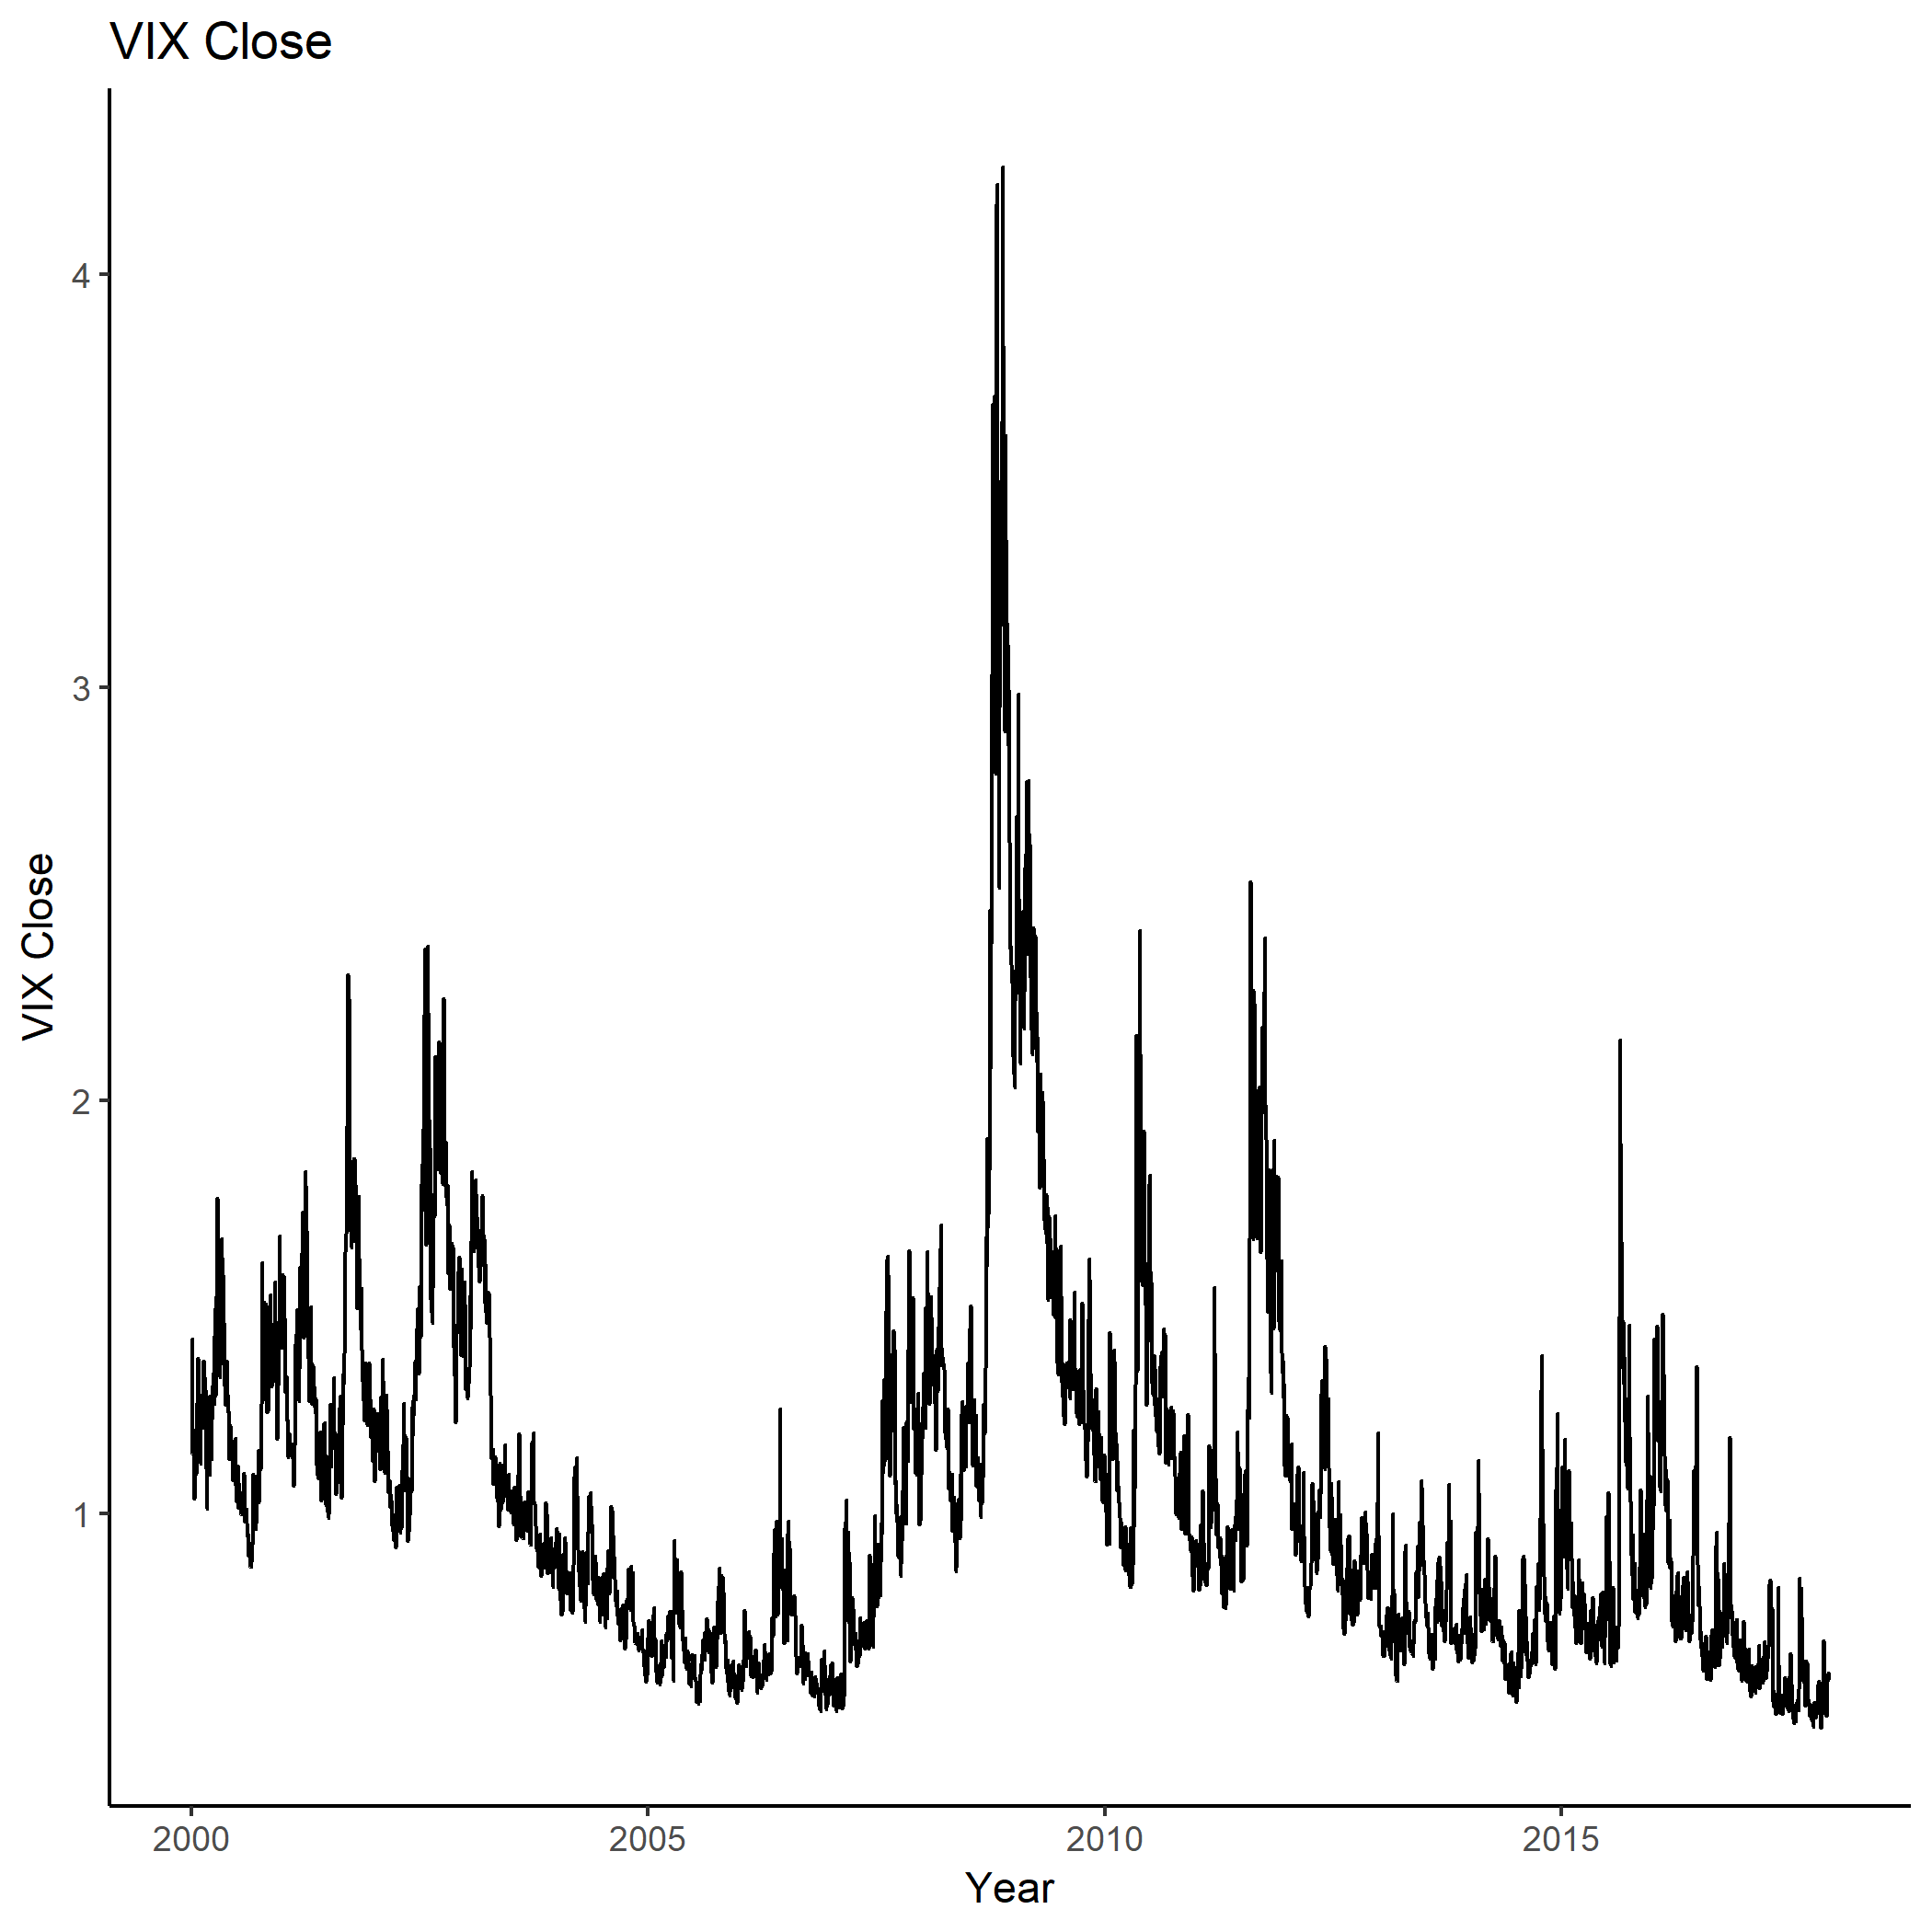
\includegraphics[width=16cm, height=8cm]{pictures/vix.png}
%\end{figure}
%
%\begin{figure}[!htbp]
%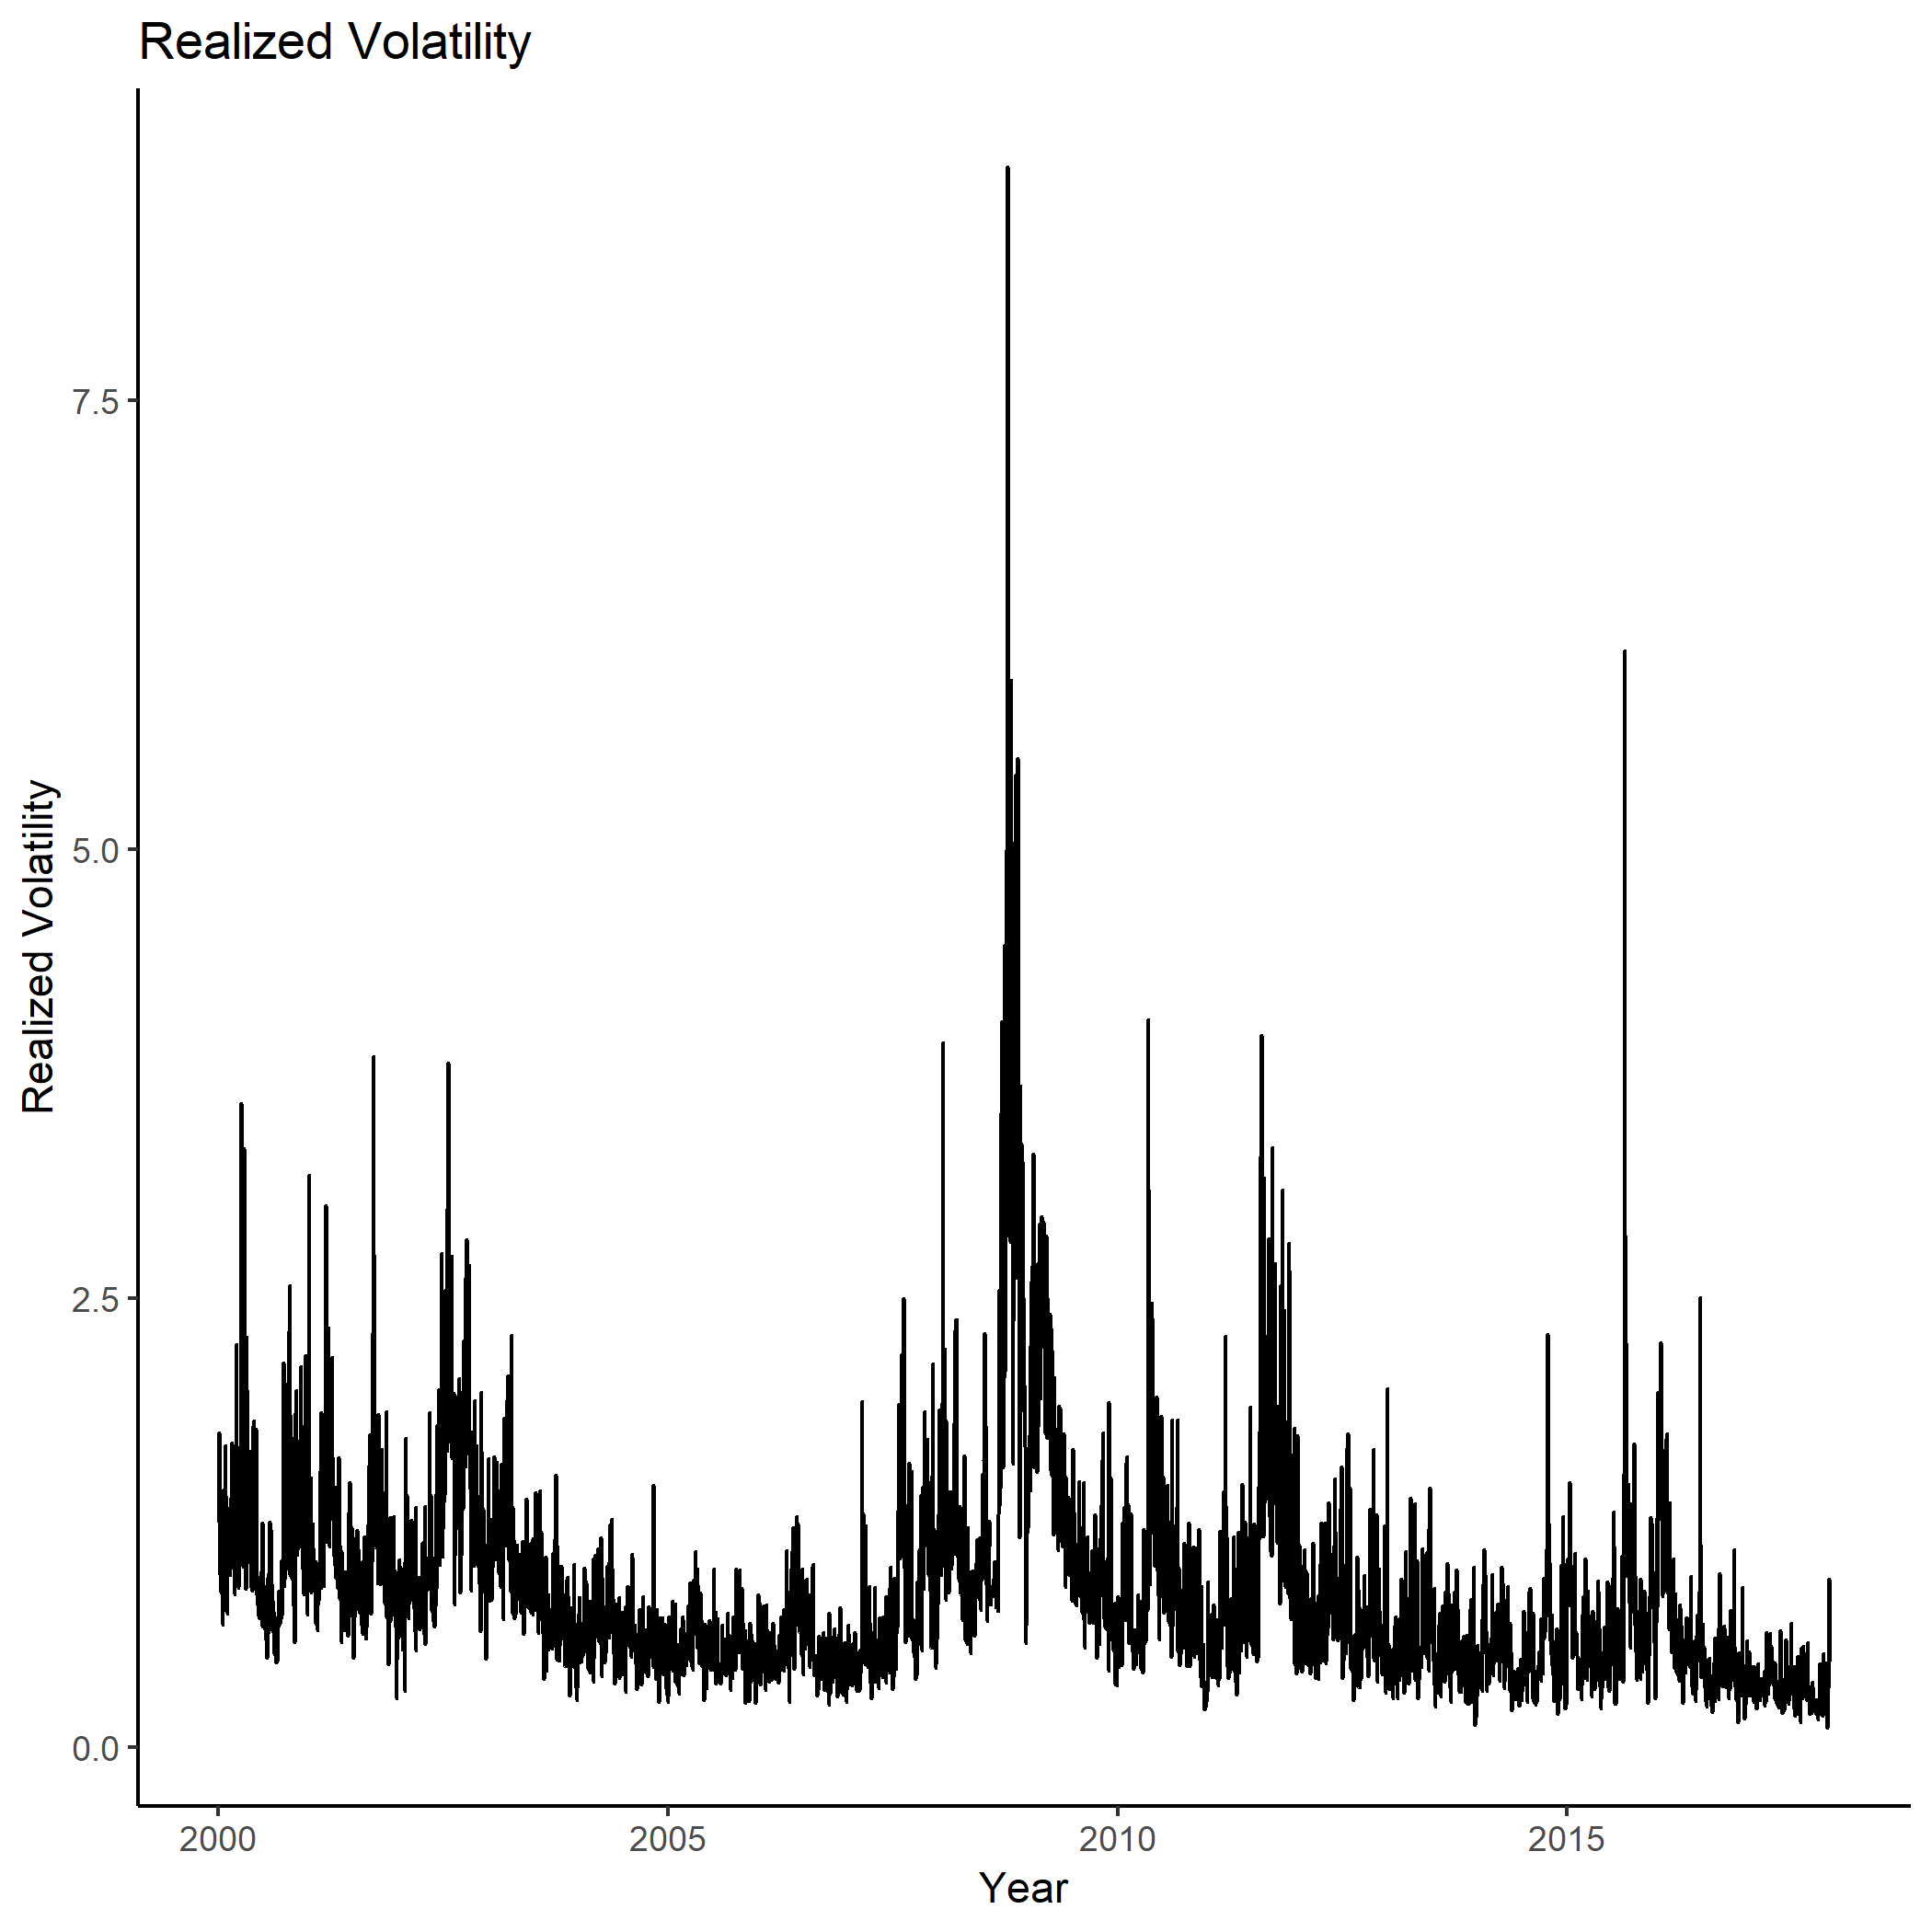
\includegraphics[width=16cm, height=8cm]{pictures/vol.png}
%\end{figure}
%
%\begin{figure}[!htbp]
%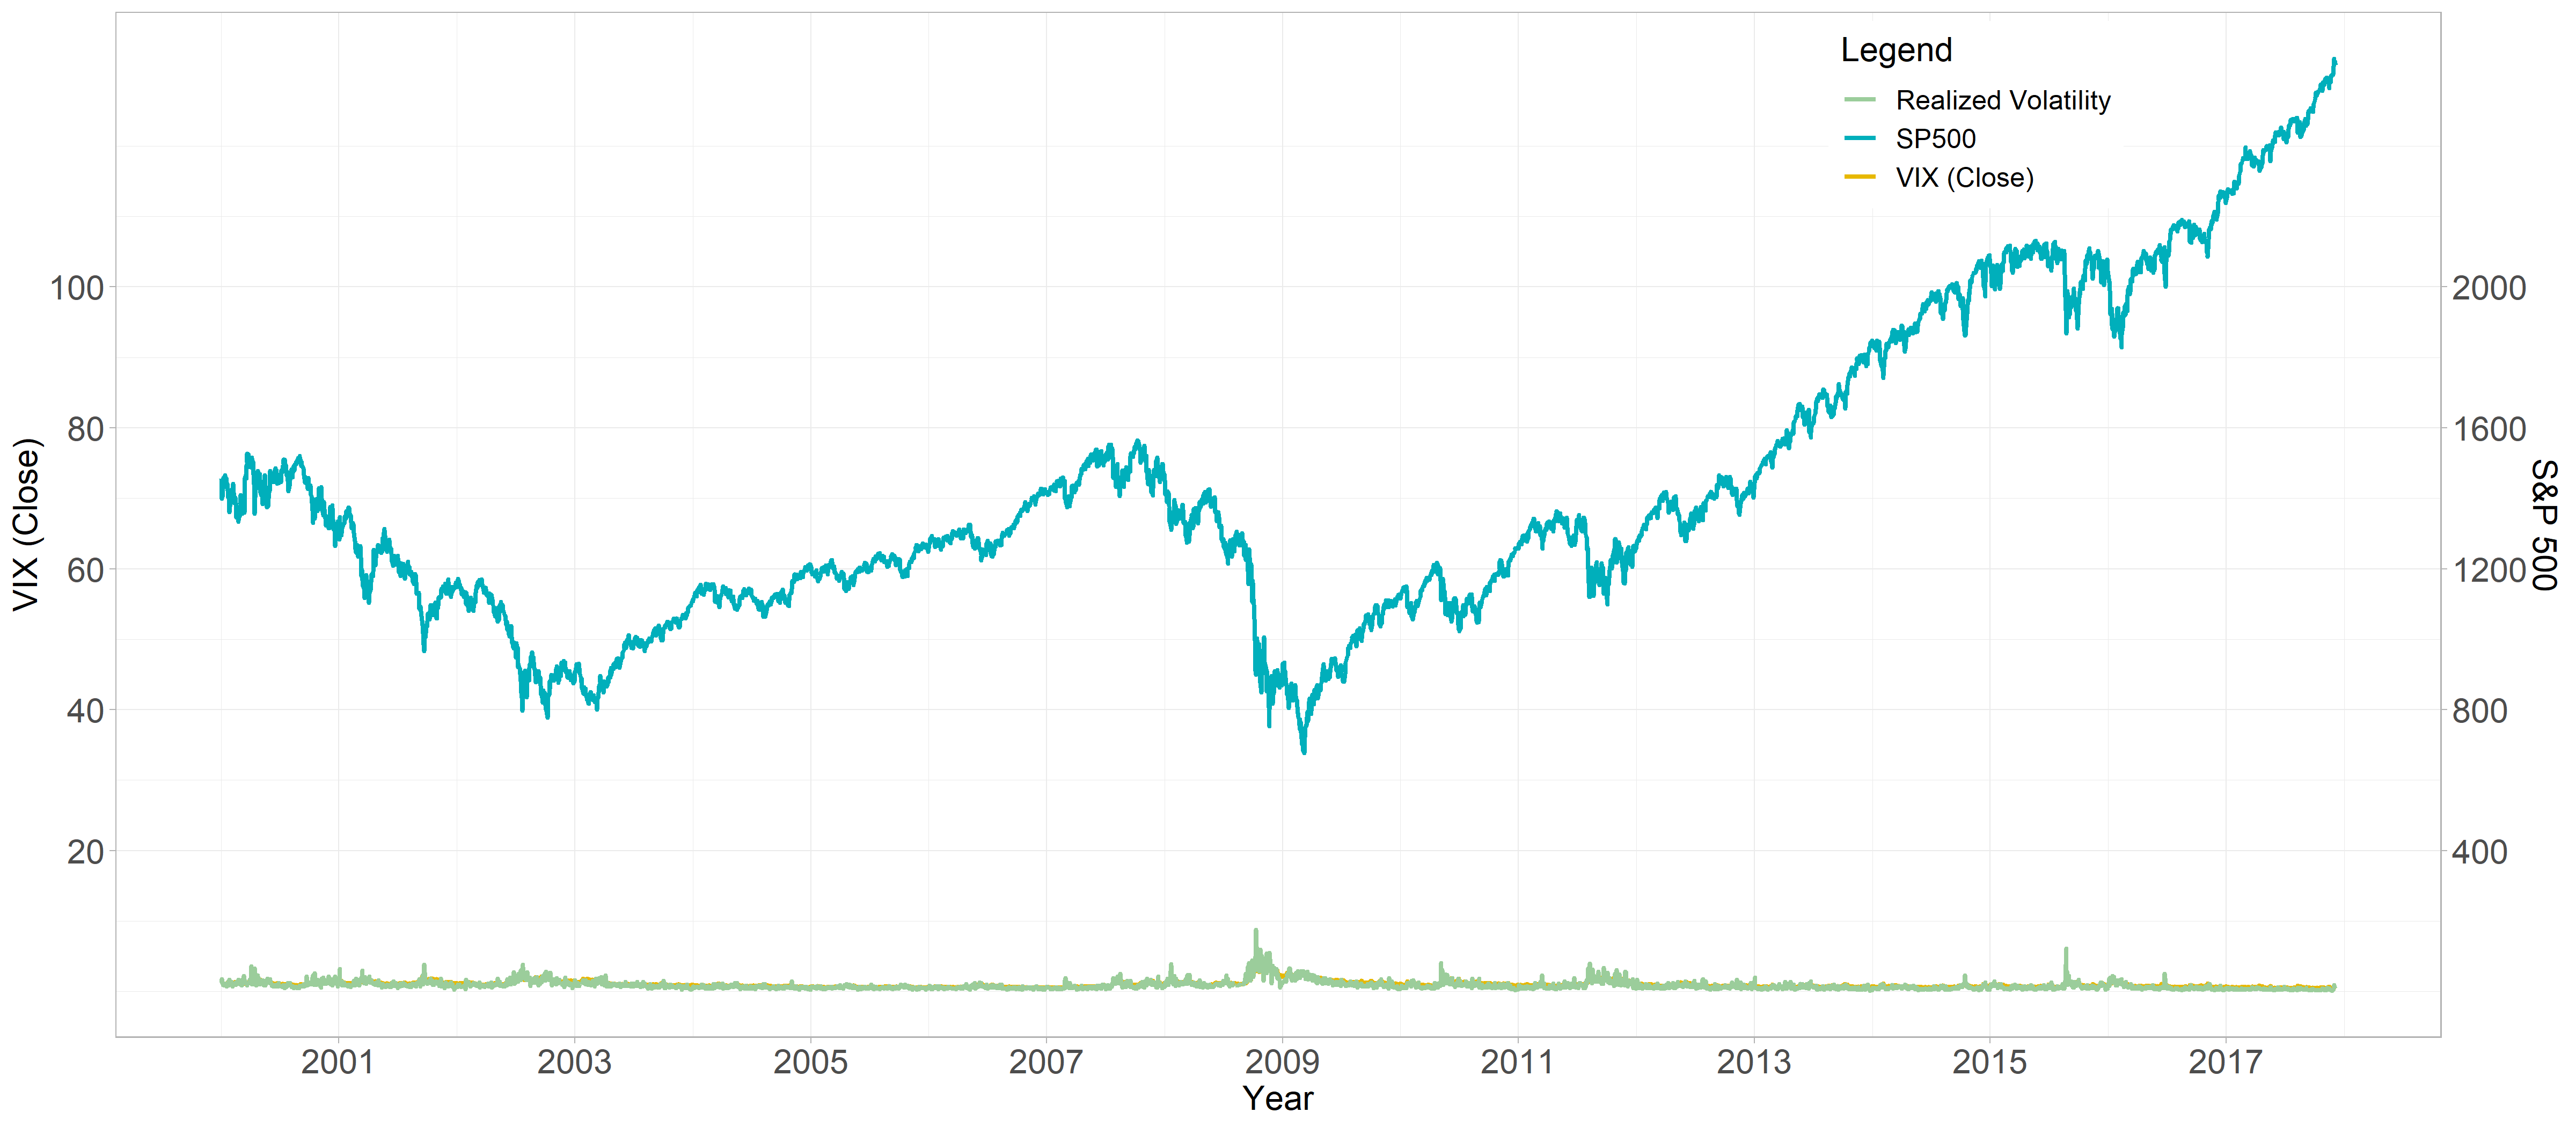
\includegraphics[width=16cm, height=8cm]{pictures/SPandVolandViX.png}
%\end{figure}

Measure for daily return variability should be realized volatility, as \citeauthor{andersen2001} suggest, that under suitable conditions it provides an unbiased estimator of the return volatility. 


\begin{itemize}\itemsep0pt
\item S\&P 500 index data on daily basis
\item sampling period: 2000 - 2018
\item realized volatility: daily realized volatility of S\&P 500, calculated using 5 minute returns, retrieved from \citeauthor{heber2009}
\item model-free implied volatility: VIX index data
\item historic volatility: lagged realized volatility, for HAR-RV model use the average over the time period used to forecast
\end{itemize}


\subsection{Limitations}
As volatility is stochastic, the ex-ante estimation will not equal the return volatility, as it is a measurement over an aggregated discrete time period \parencite{andersen2001}.
